In order to make websites more dynamic and eliminate the break of the site by loading a new \gls{html} file from the server, many ideas have been shaped and one pattern that solves this problem efficiently is the \gls{mvu} application pattern.
In order to solve the problem of showing diverged information in an \gls{html} document, the JavaScript language needs to be used, as there is no native and complex enough support for \gls{html} or \gls{css} to force the browser to show this new information. JavaScript on the other hand can directly inject into the \gls{dom}, by having complete access to every \gls{html} node element in the rendered \gls{dom}.
JavaScript can select a node element by \texttt{ID} and change its displayed value, forcing the browser to rerender the \gls{dom} on that node. Figure \ref{fig:button_browser} shows a minimal example, where JavaScript is used to alter the rendered \gls{html}.

\begin{figure}
    \centering
    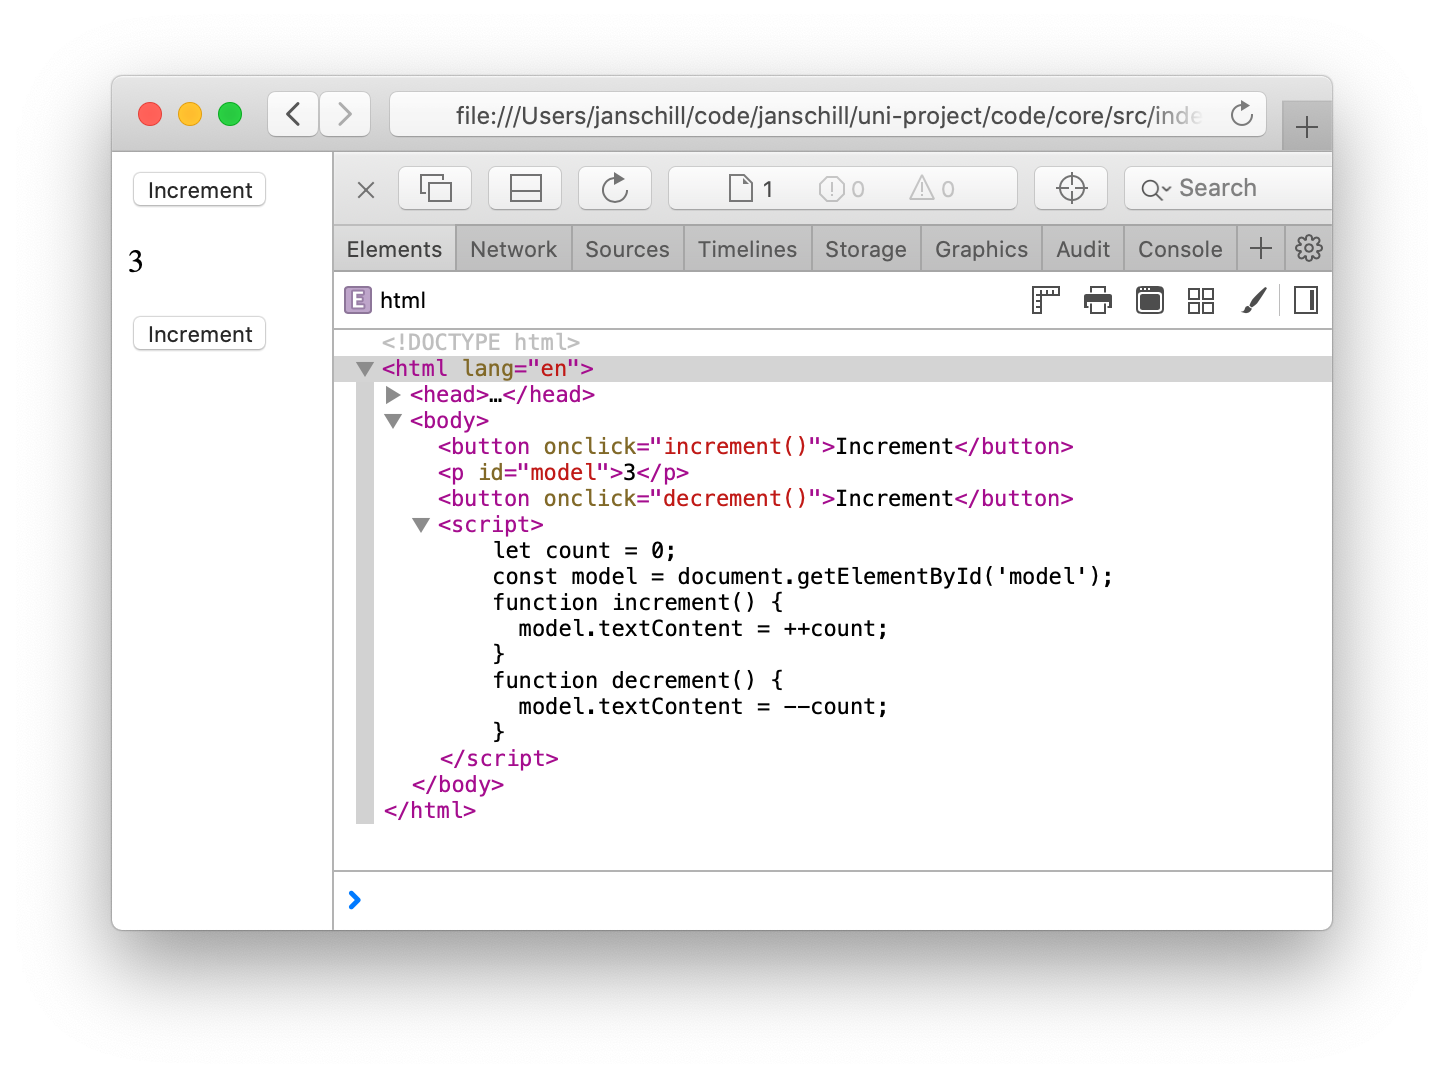
\includegraphics[width=0.8\textwidth]{images/button-browser.png}
    \caption{Simple button counter example}
    \label{fig:button_browser}
\end{figure}

This way of updating content on the document directly has been evolved over the years and is heavily used to build any sized modern websites. With the help of frameworks like React, a JavaScript framework developed by Facebook or Elm a framework that uses its own functional language, it has become easier to go from a small button example to a fully working componentized website.
The Elm framework uses the \gls{mvu} application pattern to realize the idea of dynamically updating the \gls{dom}.

The basic functionality how Elm uses it, is that it generates \gls{html} that can be viewed by a client. This client can then interact with the \gls{html} by clicking a button for example, producing a \texttt{Msg (Message)}, which is send to Elm, producing another \gls{html} document.
In the Elm program three parts play a crucial role: the Model, View and Update.

When a message of type \texttt{Msg} is produced, the update function is being called, which takes the message sent and the current state of the model, returning an updated model. The view function, responsible of generating the \gls{html} that can be views by the browser is called automatically, rendering the \gls{html} with the updated model.

\begin{verbatim}
view : Model -> Html Msg
update : Msg -> Model -> Model
\end{verbatim}

\paragraph{How does Elm optimise the view rendering?}
Because most of the time when a new view was generated and needs re-rendered, it is not necessary for the whole document to be switched out, but rather only the \gls{dom} node that experienced change -- forcing the browser to generate new \gls{dom} nodes is computational expensive work.
For this most frameworks use a \gls{vdom}, which resembles the complete active \gls{dom} in memory in a convenient data structure. This \gls{vdom} is then generated with the updated model and compared against the current active \gls{vdom}, finding the parts that need updating. This part is called \textit{diffing} and it is done by iterating over both representations of the \gls{dom} and comparing each individual node. This \textit{diffing} then generates a data structure that keeps track of all changes. A \textit{patch} function, taking the old view and the data structure holding the changes, then generates a representation of the new view by switching out all the nodes that need updating.

All the \textit{diffing} and \textit{patching} against the whole \gls{dom} tree seems to be still computational expensive, when in the end for the button example only the following is needed:

\begin{figure}[]
    \centering
\begin{verbatim}
<html>
  <button onclick=increment()>Increment</button>
  <p id="model">0</p>
</html>
<script>
  let count = 0;
  const model = document.getElementById('model');
  function increment() {
    model.textContent = ++count;
  }
</script>
\end{verbatim}
    \caption{Reduced example to show only the incrementing}
    \label{fig:button-increment}
\end{figure}

\paragraph{How does JaLi optimize the view rendering even further?} This paper will outline all the needed parts to use partial evaluation, symbolic execution and constant folding to optimize the view rendering. It will be shown on the small button example how the compiler of the JaLi language can reduce all the previously mentioned parts that are computational expensive, by applying the optimizations.
Due to time restrictions it was not able to implement the full working compiler optimizations, nor a compiler that transforms a full program to a \gls{html} and JavaScript website that could be run in the browser. Nevertheless the theory has been established and it will be shown on small examples to illustrate the idea.